% =========================================================
% CHAPTER 8: SYSTEM DESIGN
% =========================================================
\chapter{System Design}
\label{chap:system_design}

\section{High-Level Architectural Overview}
FraudShield AI is designed around a 5-tier layered architecture that decouples user interfaces, RESTful API controllers, business security logic, machine learning inference engines, and persistent data storage.

\begin{figure}[htbp]
    \centering
    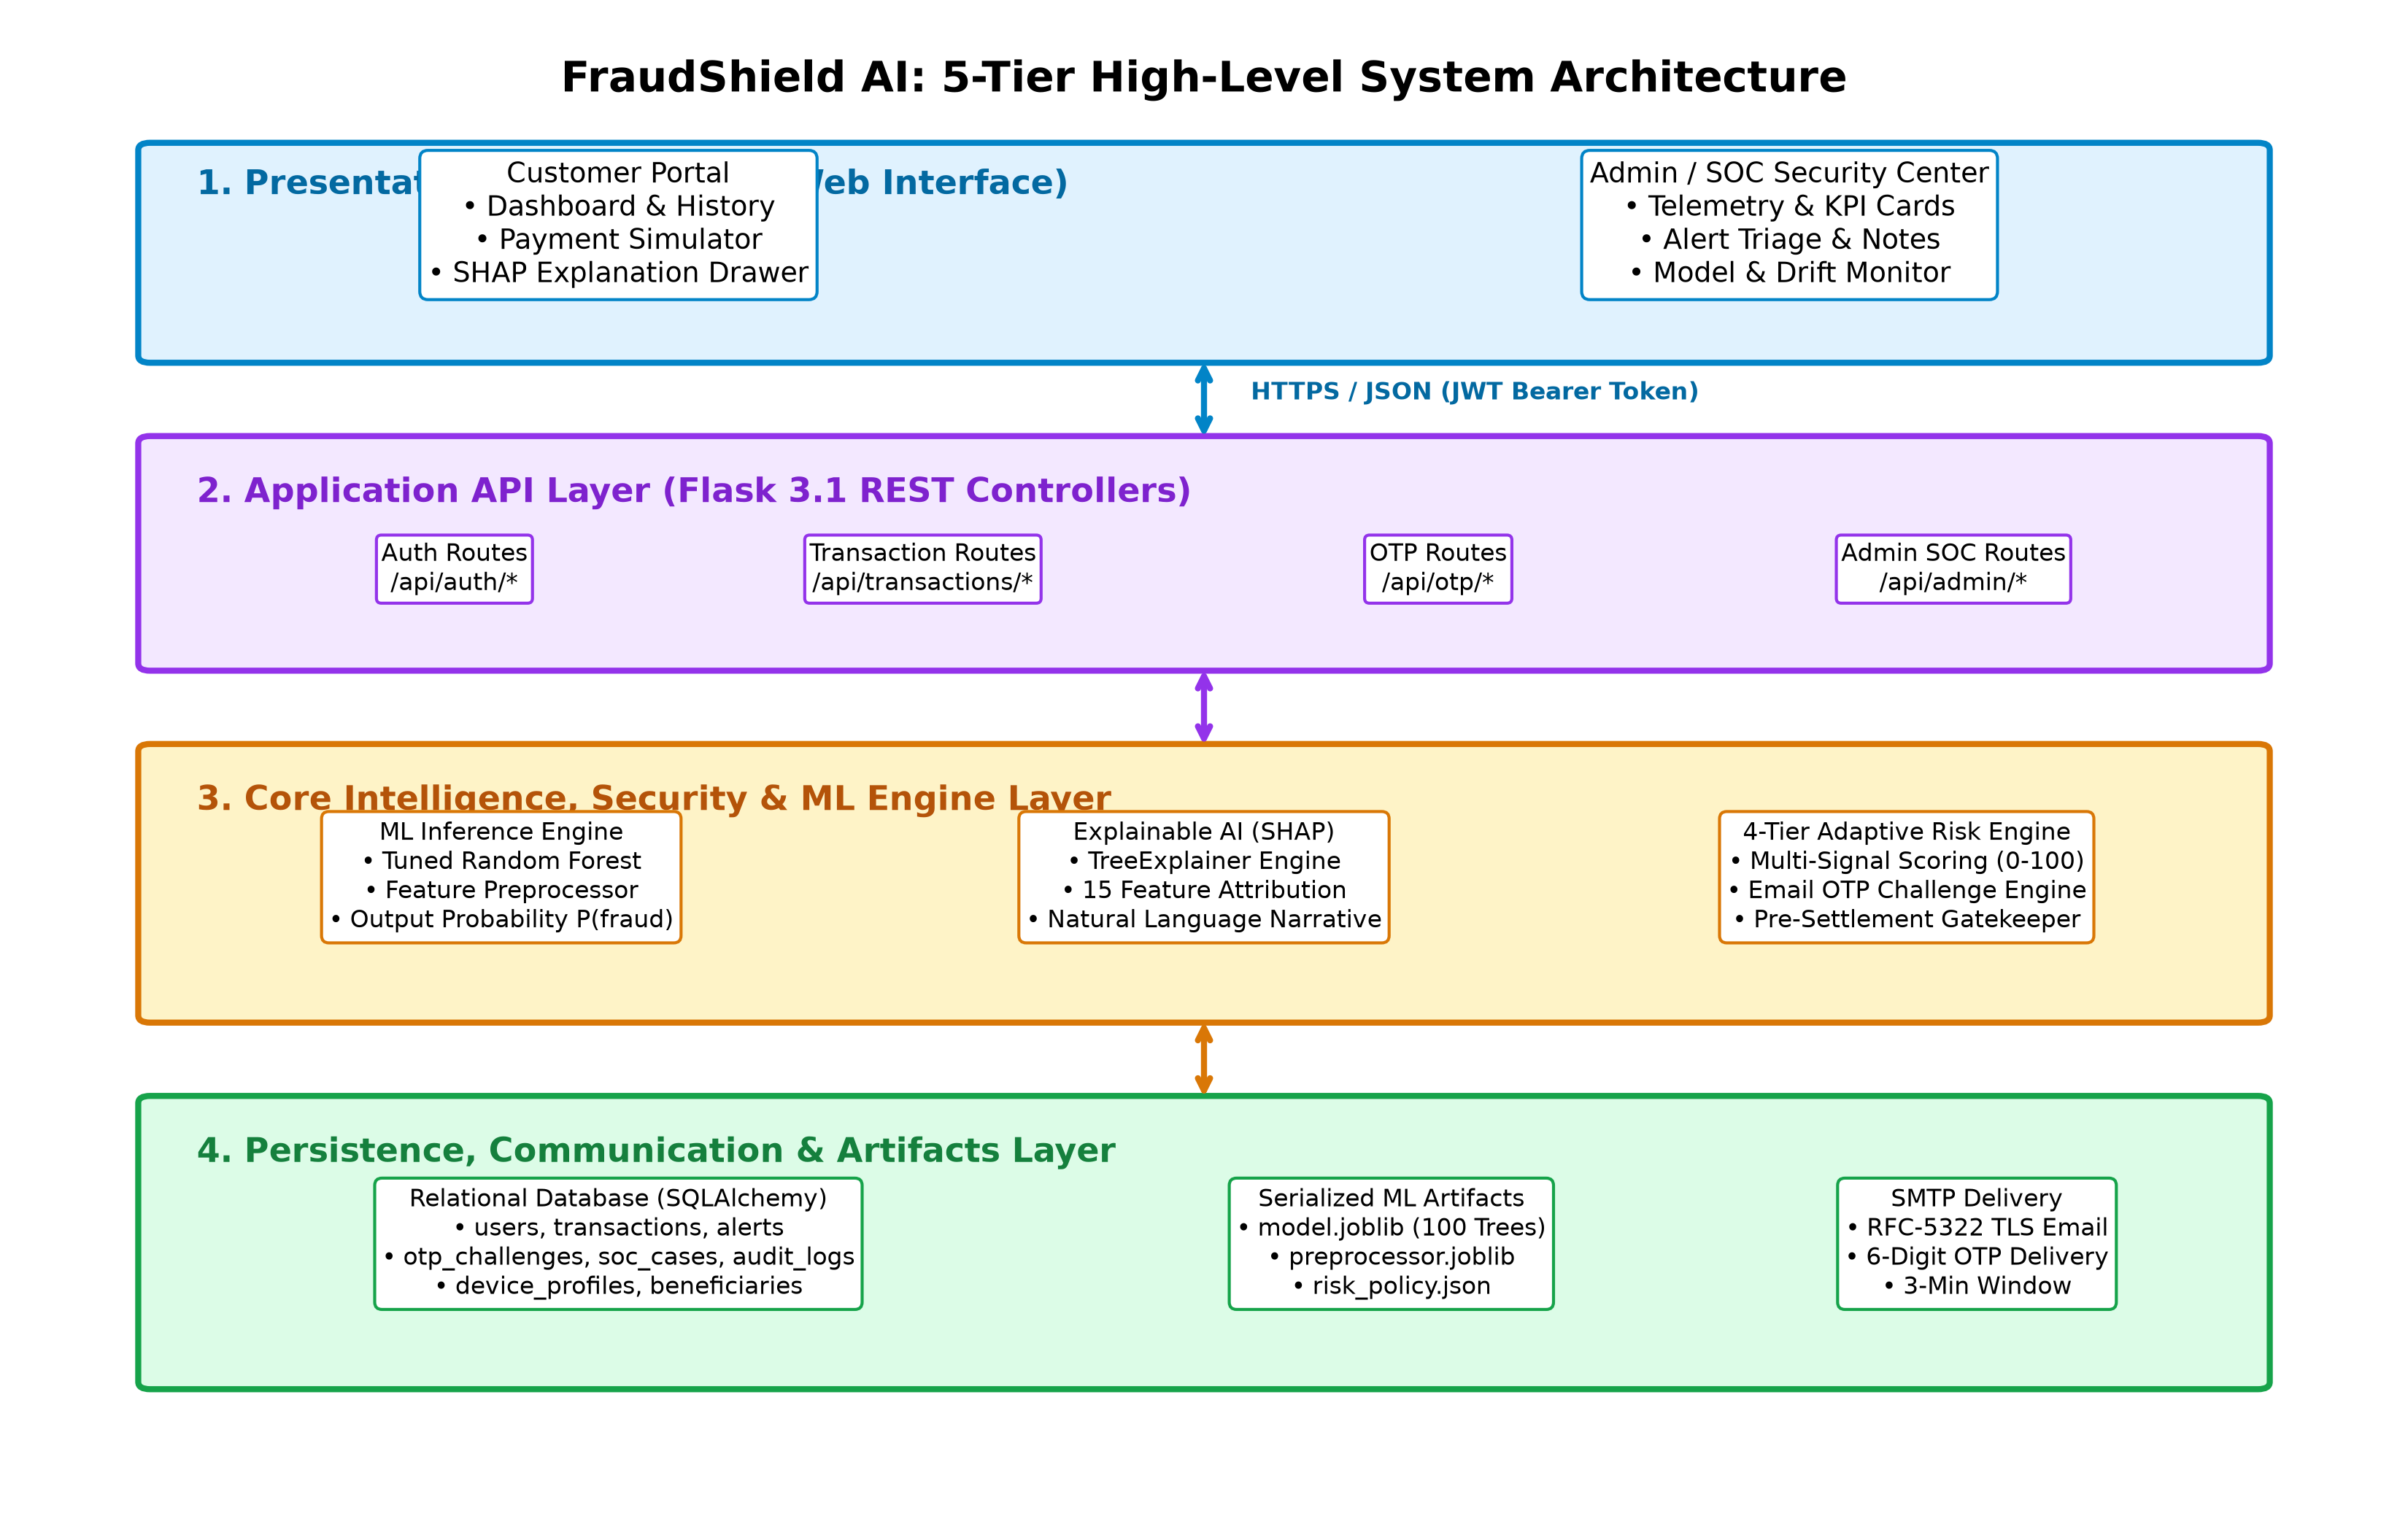
\includegraphics[width=0.92\textwidth]{figures/architecture_diagram.png}
    \caption{FraudShield AI: 5-Tier High-Level System Architecture}
    \label{fig:architecture_diagram}
\end{figure}

The architectural layers operate as follows:
\begin{enumerate}[label=\arabic*.]
    \item \textbf{Presentation Layer}: Delivers responsive client interfaces for both retail customers (payment simulator, dashboard, SHAP drawer) and SOC security officers (alert triage, KPIs, feature drift telemetry).
    \item \textbf{Application API Layer}: Exposes RESTful HTTP endpoints organized into Flask Blueprints (\texttt{auth\_routes}, \texttt{transaction\_routes}, \texttt{otp\_routes}, \texttt{admin\_routes}).
    \item \textbf{Business Logic \& Security Layer}: Implements core domain logic, PIN validation, beneficiary management, and rate limiting.
    \item \textbf{Machine Learning \& Explainability Layer}: Houses the serialized Random Forest model, feature engineering transforms, and the SHAP TreeExplainer.
    \item \textbf{Persistence \& Artifacts Layer}: Manages relational database storage (SQLAlchemy) and physical ML joblib artifacts.
\end{enumerate}

\section{End-to-End System Transaction Workflow}
The transaction lifecycle follows a strict sequence to ensure that fraud detection occurs \textbf{prior} to any financial settlement:

\begin{figure}[htbp]
    \centering
    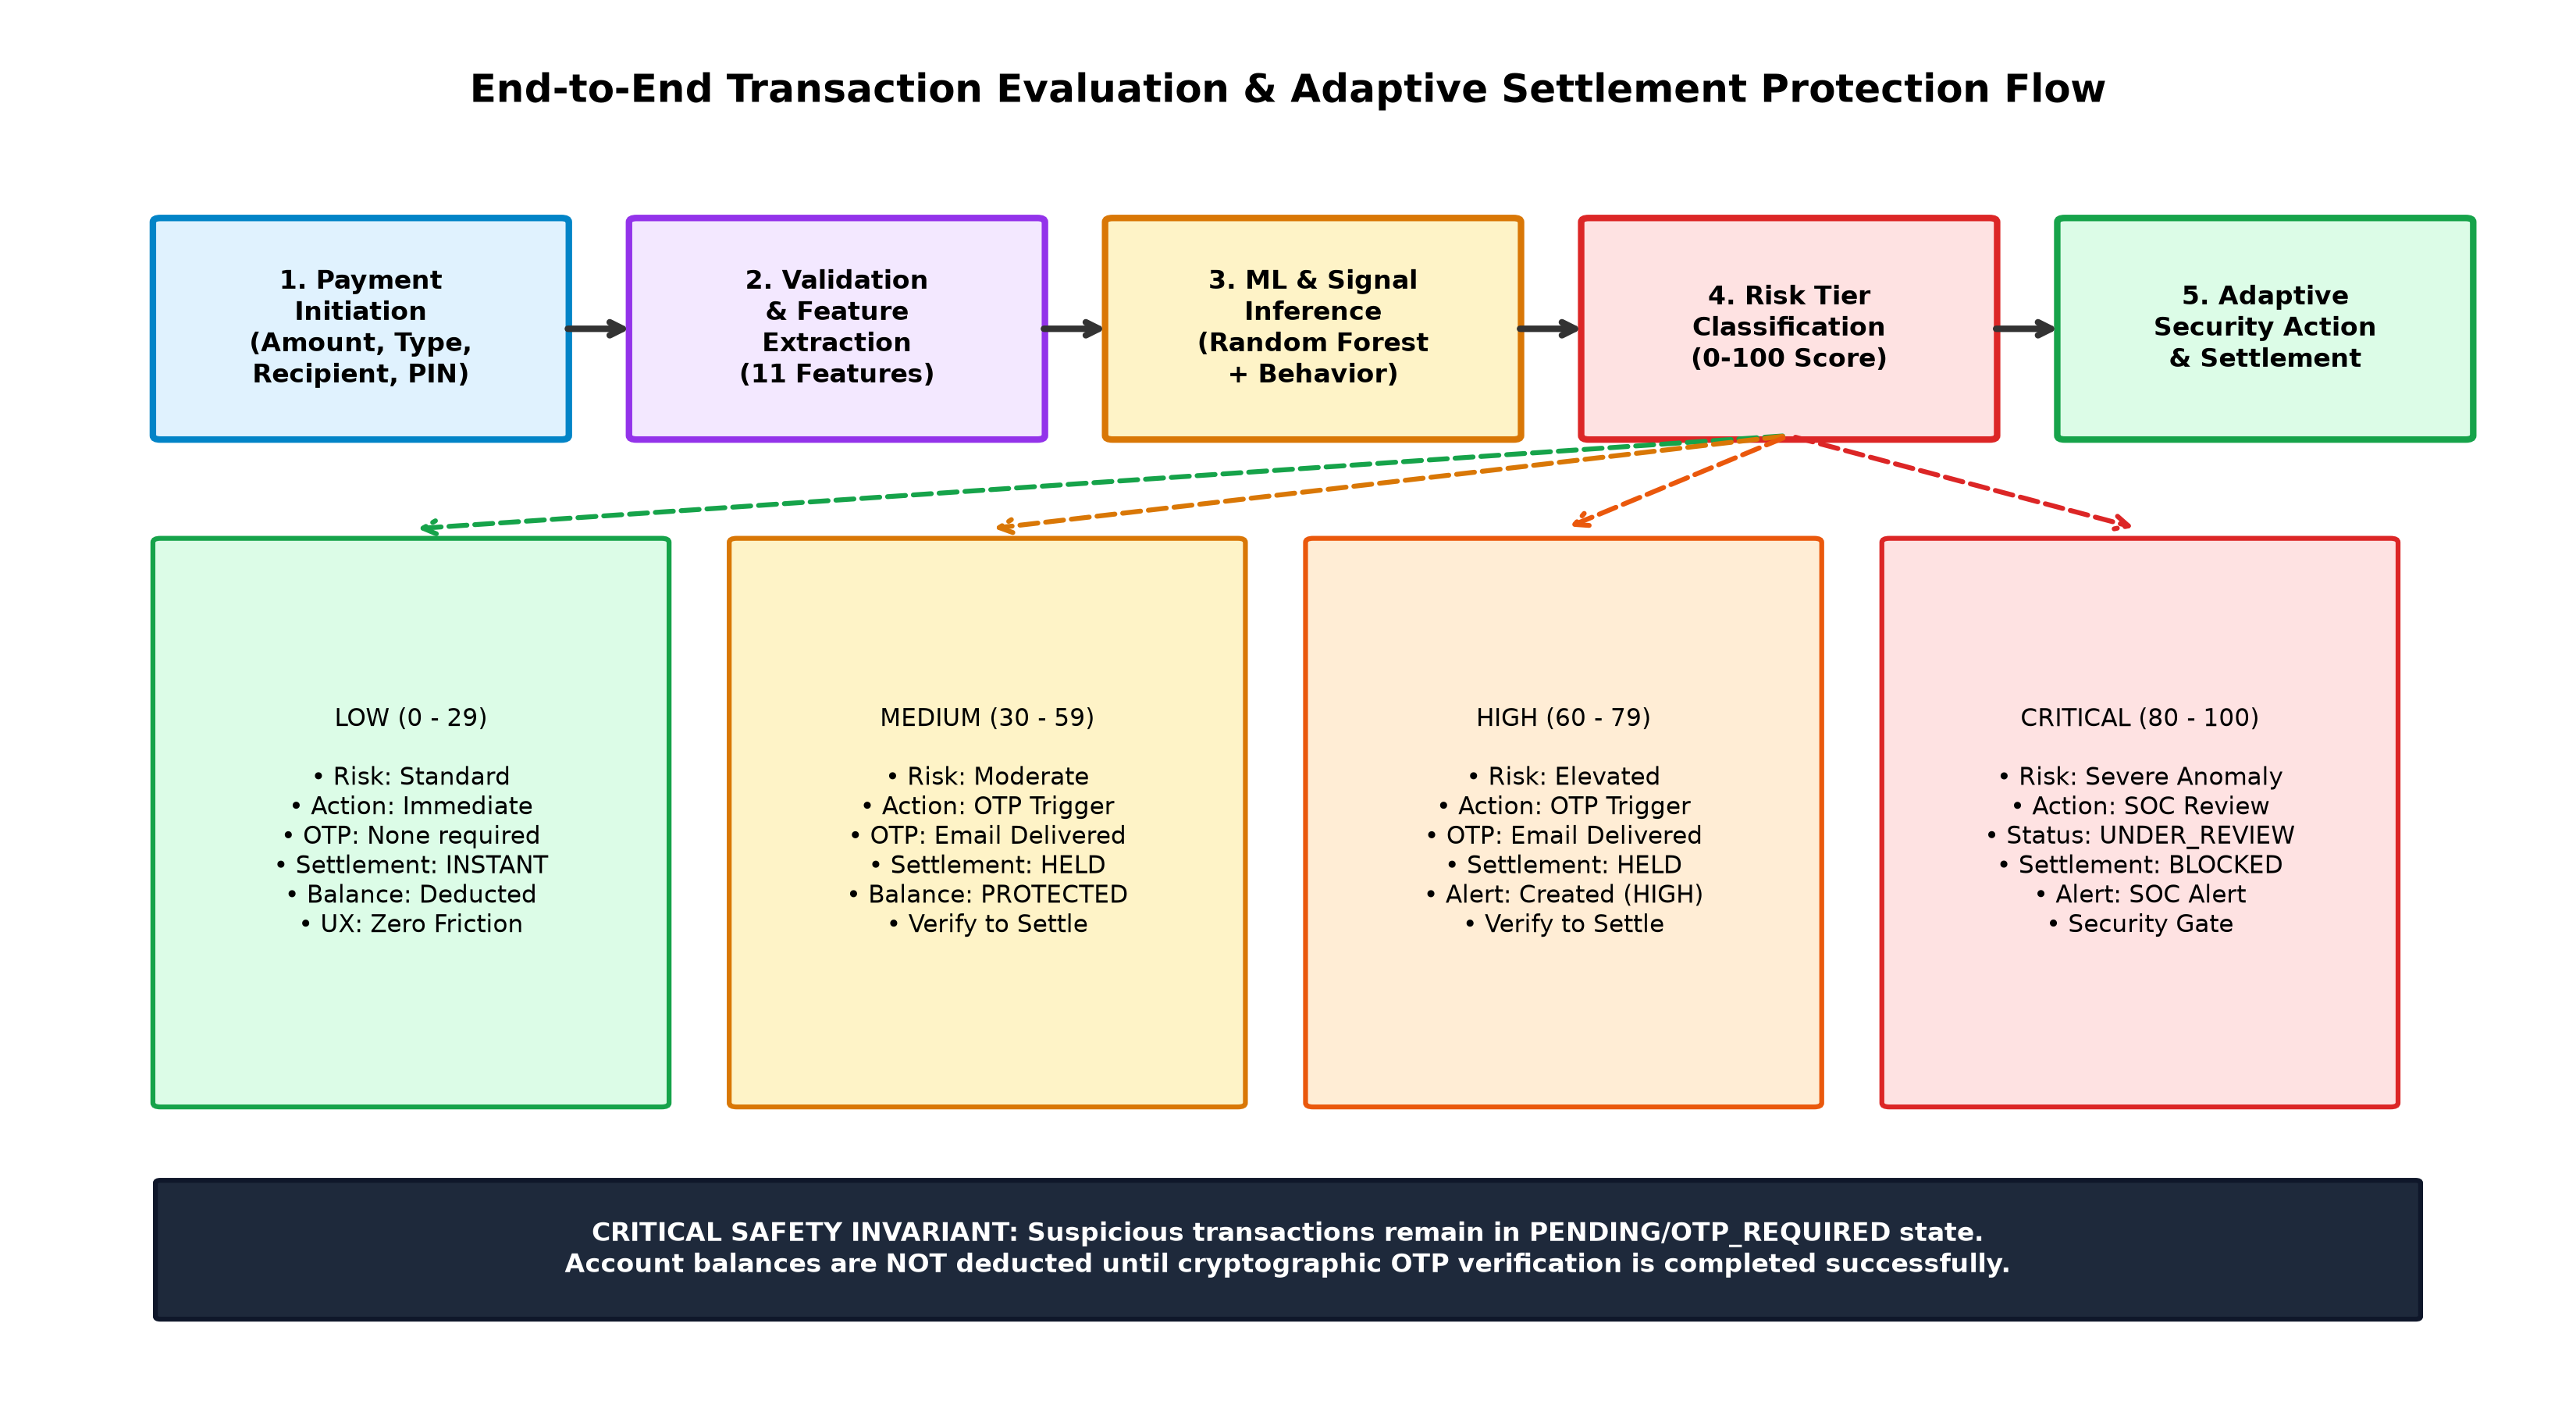
\includegraphics[width=0.95\textwidth]{figures/risk_workflow_diagram.png}
    \caption{End-to-End Transaction Evaluation and Adaptive Settlement Protection Workflow}
    \label{fig:risk_workflow_diagram}
\end{figure}

The chronological execution steps are:
\begin{enumerate}[label=\textbf{Step \arabic*:}]
    \item \textbf{Transaction Initiation}: Customer submits payment payload (recipient VPA/phone, amount, transfer type, 4--6 digit numeric PIN) via the web interface.
    \item \textbf{Authentication \& Account Validation}: Backend verifies active JWT token, validates PIN against stored cryptographic hash, checks account lockout counters, and confirms sufficient balance.
    \item \textbf{Feature Engineering}: Extracts 11 logical transaction properties and computes engineered behavioral indicators:
    \begin{align}
        \text{errorBalanceOrig} &= \text{oldbalanceOrg} - \text{newbalanceOrig} - \text{amount} \\
        \text{errorBalanceDest} &= \text{oldbalanceDest} + \text{amount} - \text{newbalanceDest} \\
        \text{amountToBalanceRatio} &= \frac{\text{amount}}{\text{oldbalanceOrg} + 1.0} \\
        \text{hourOfDay} &= \text{step} \pmod{24}
    \end{align}
    \item \textbf{ML Inference \& SHAP Attribution}: Model preprocessor transforms features into a 15-dimensional vector; Random Forest computes $P(\text{fraud})$; SHAP calculates exact feature Shapley values.
    \item \textbf{4-Tier Risk Classification}: System calculates combined risk score ($0-100$) and assigns risk tier (\textit{LOW, MEDIUM, HIGH, CRITICAL}).
    \item \textbf{Adaptive Security Action}:
    \begin{itemize}
        \item \textit{LOW ($0-29$)}: Instantly approved; sender balance deducted; recipient credited; status \texttt{APPROVED}.
        \item \textit{MEDIUM ($30-59$)}: Held in \texttt{OTP\_REQUIRED}; zero balance deducted; 6-digit Email OTP delivered.
        \item \textit{HIGH ($60-79$)}: Held in \texttt{OTP\_REQUIRED}; zero balance deducted; Email OTP delivered; security alert opened.
        \item \textit{CRITICAL ($80-100$)}: Routed to \texttt{UNDER\_REVIEW}; balance locked; SOC security case opened.
    \end{itemize}
    \item \textbf{OTP Verification \& Final Settlement}: Upon entering valid Email OTP within 180 seconds, atomic settlement executes, updating balances and marking the transaction \texttt{SETTLED}.
\end{enumerate}

\section{Data Flow Diagrams (DFD)}

\subsection{DFD Level 0 — Context Diagram}
Figure~\ref{fig:dfd_level0} illustrates the Level 0 Context Diagram representing external entities interacting with the core platform boundaries.

\begin{figure}[htbp]
    \centering
    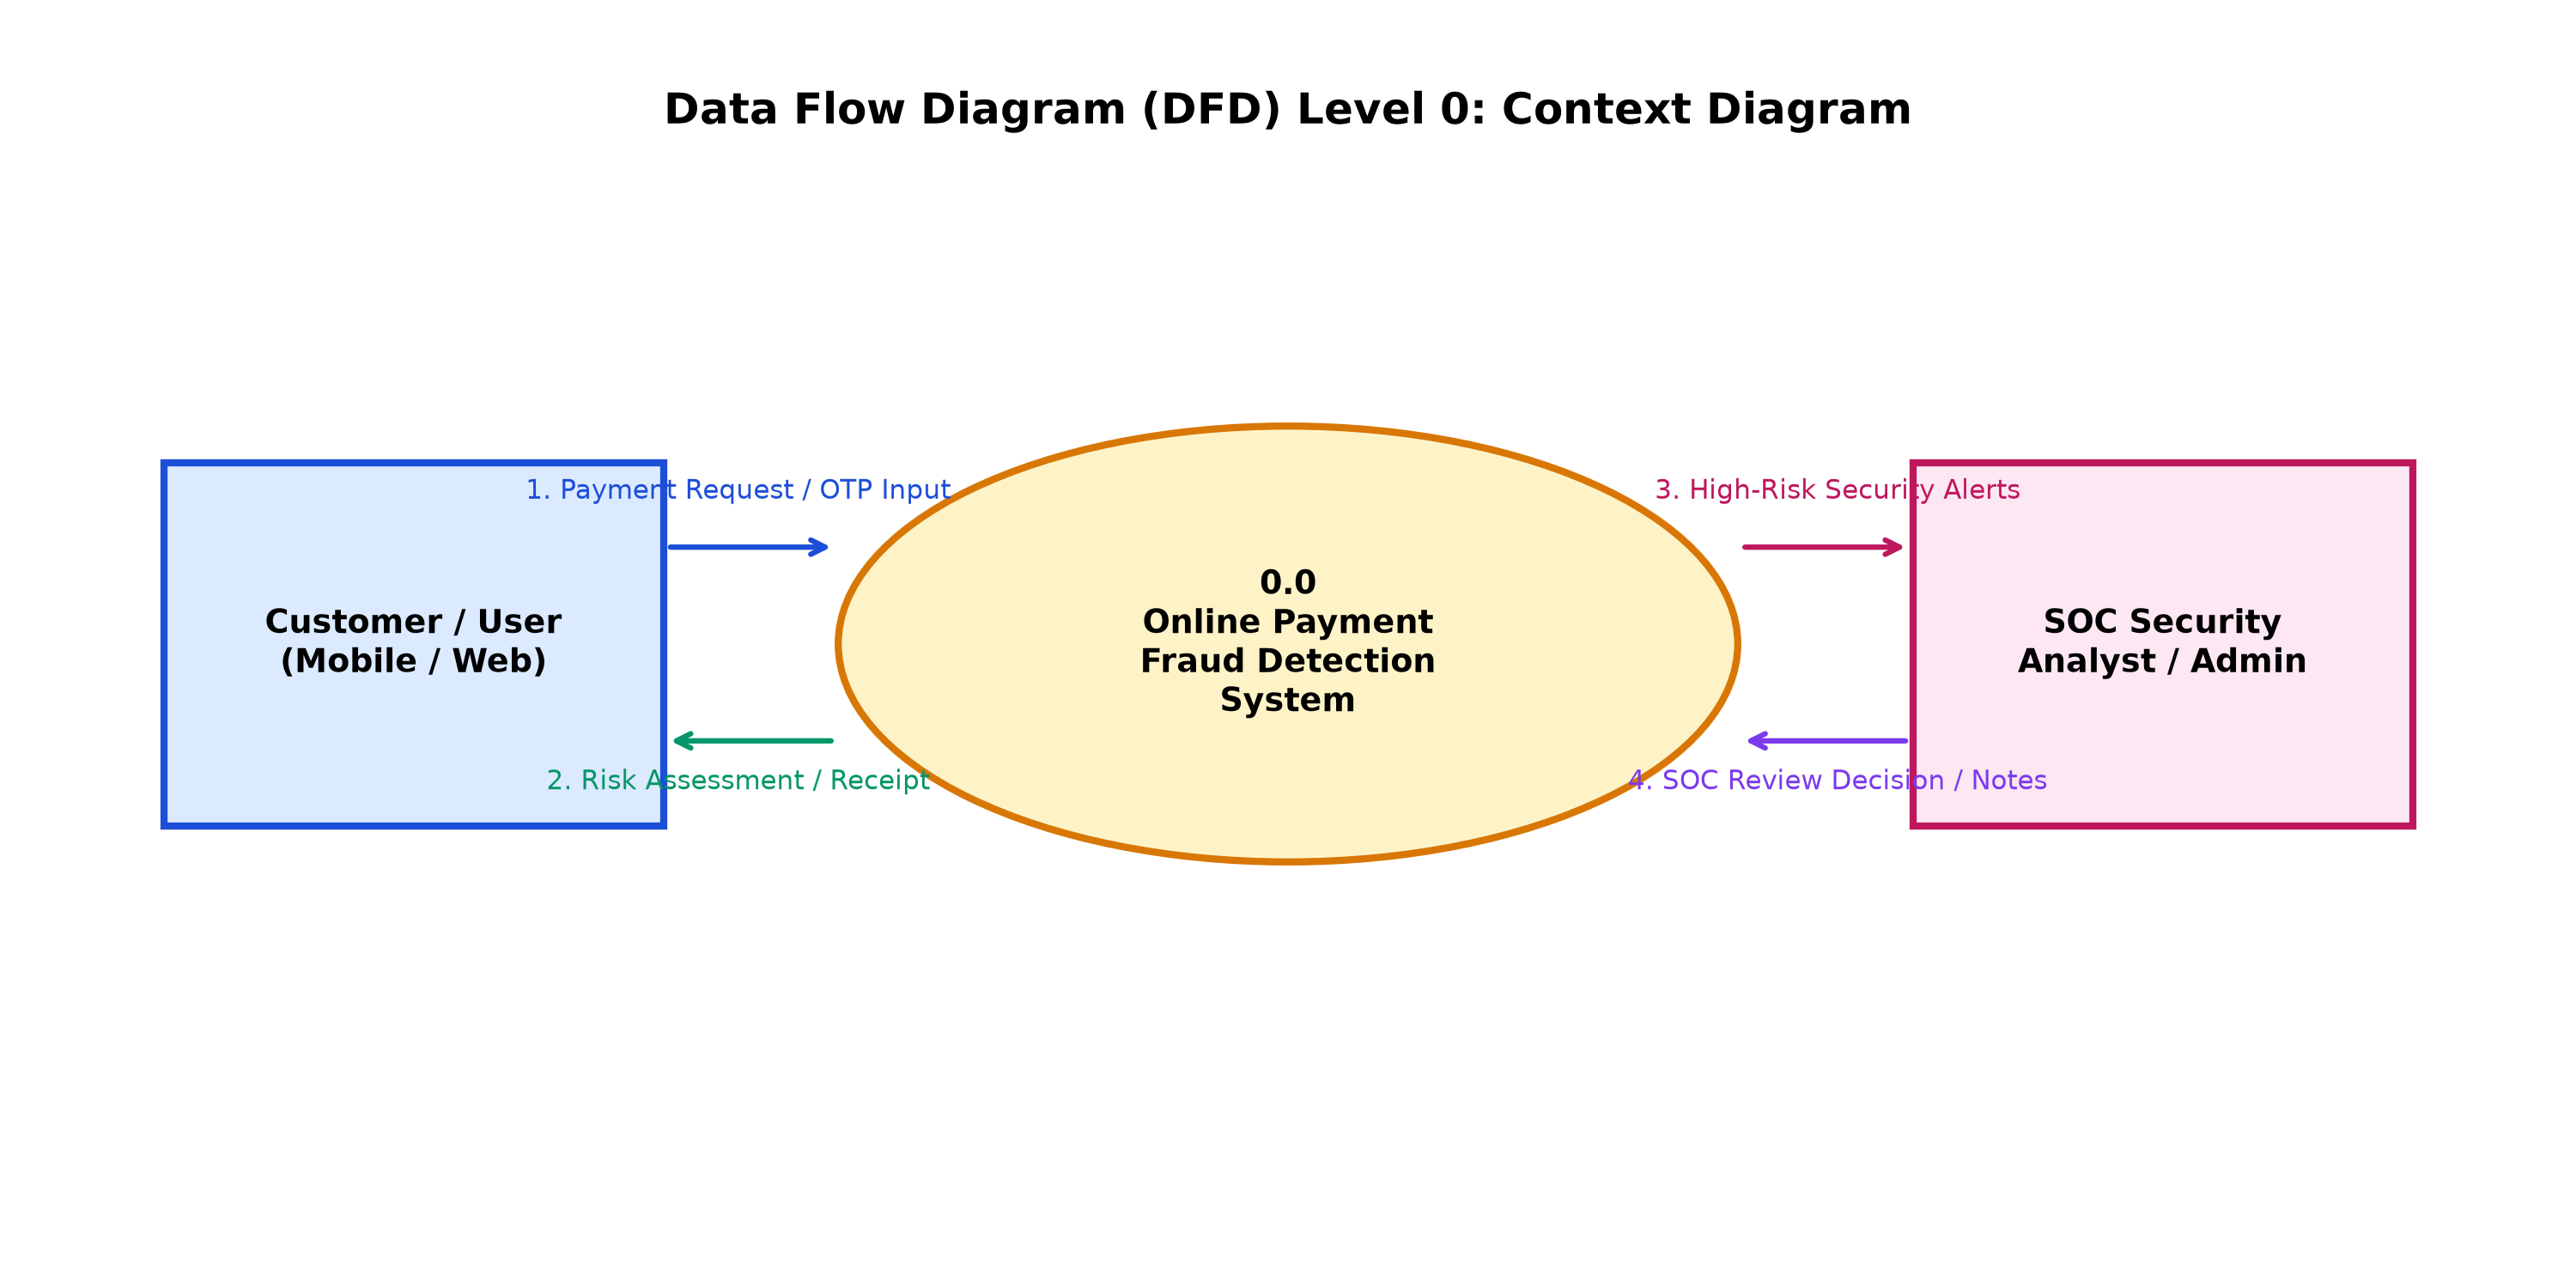
\includegraphics[width=0.85\textwidth]{figures/dfd_level0.png}
    \caption{DFD Level 0: System Context Diagram}
    \label{fig:dfd_level0}
\end{figure}

\subsection{DFD Level 1 — Subsystem Data Flow Diagram}
Figure~\ref{fig:dfd_level1} details the Level 1 functional processes, data stores (D1: Relational Database, D2: ML Artifacts), and data flow pathways across subsystems.

\begin{figure}[htbp]
    \centering
    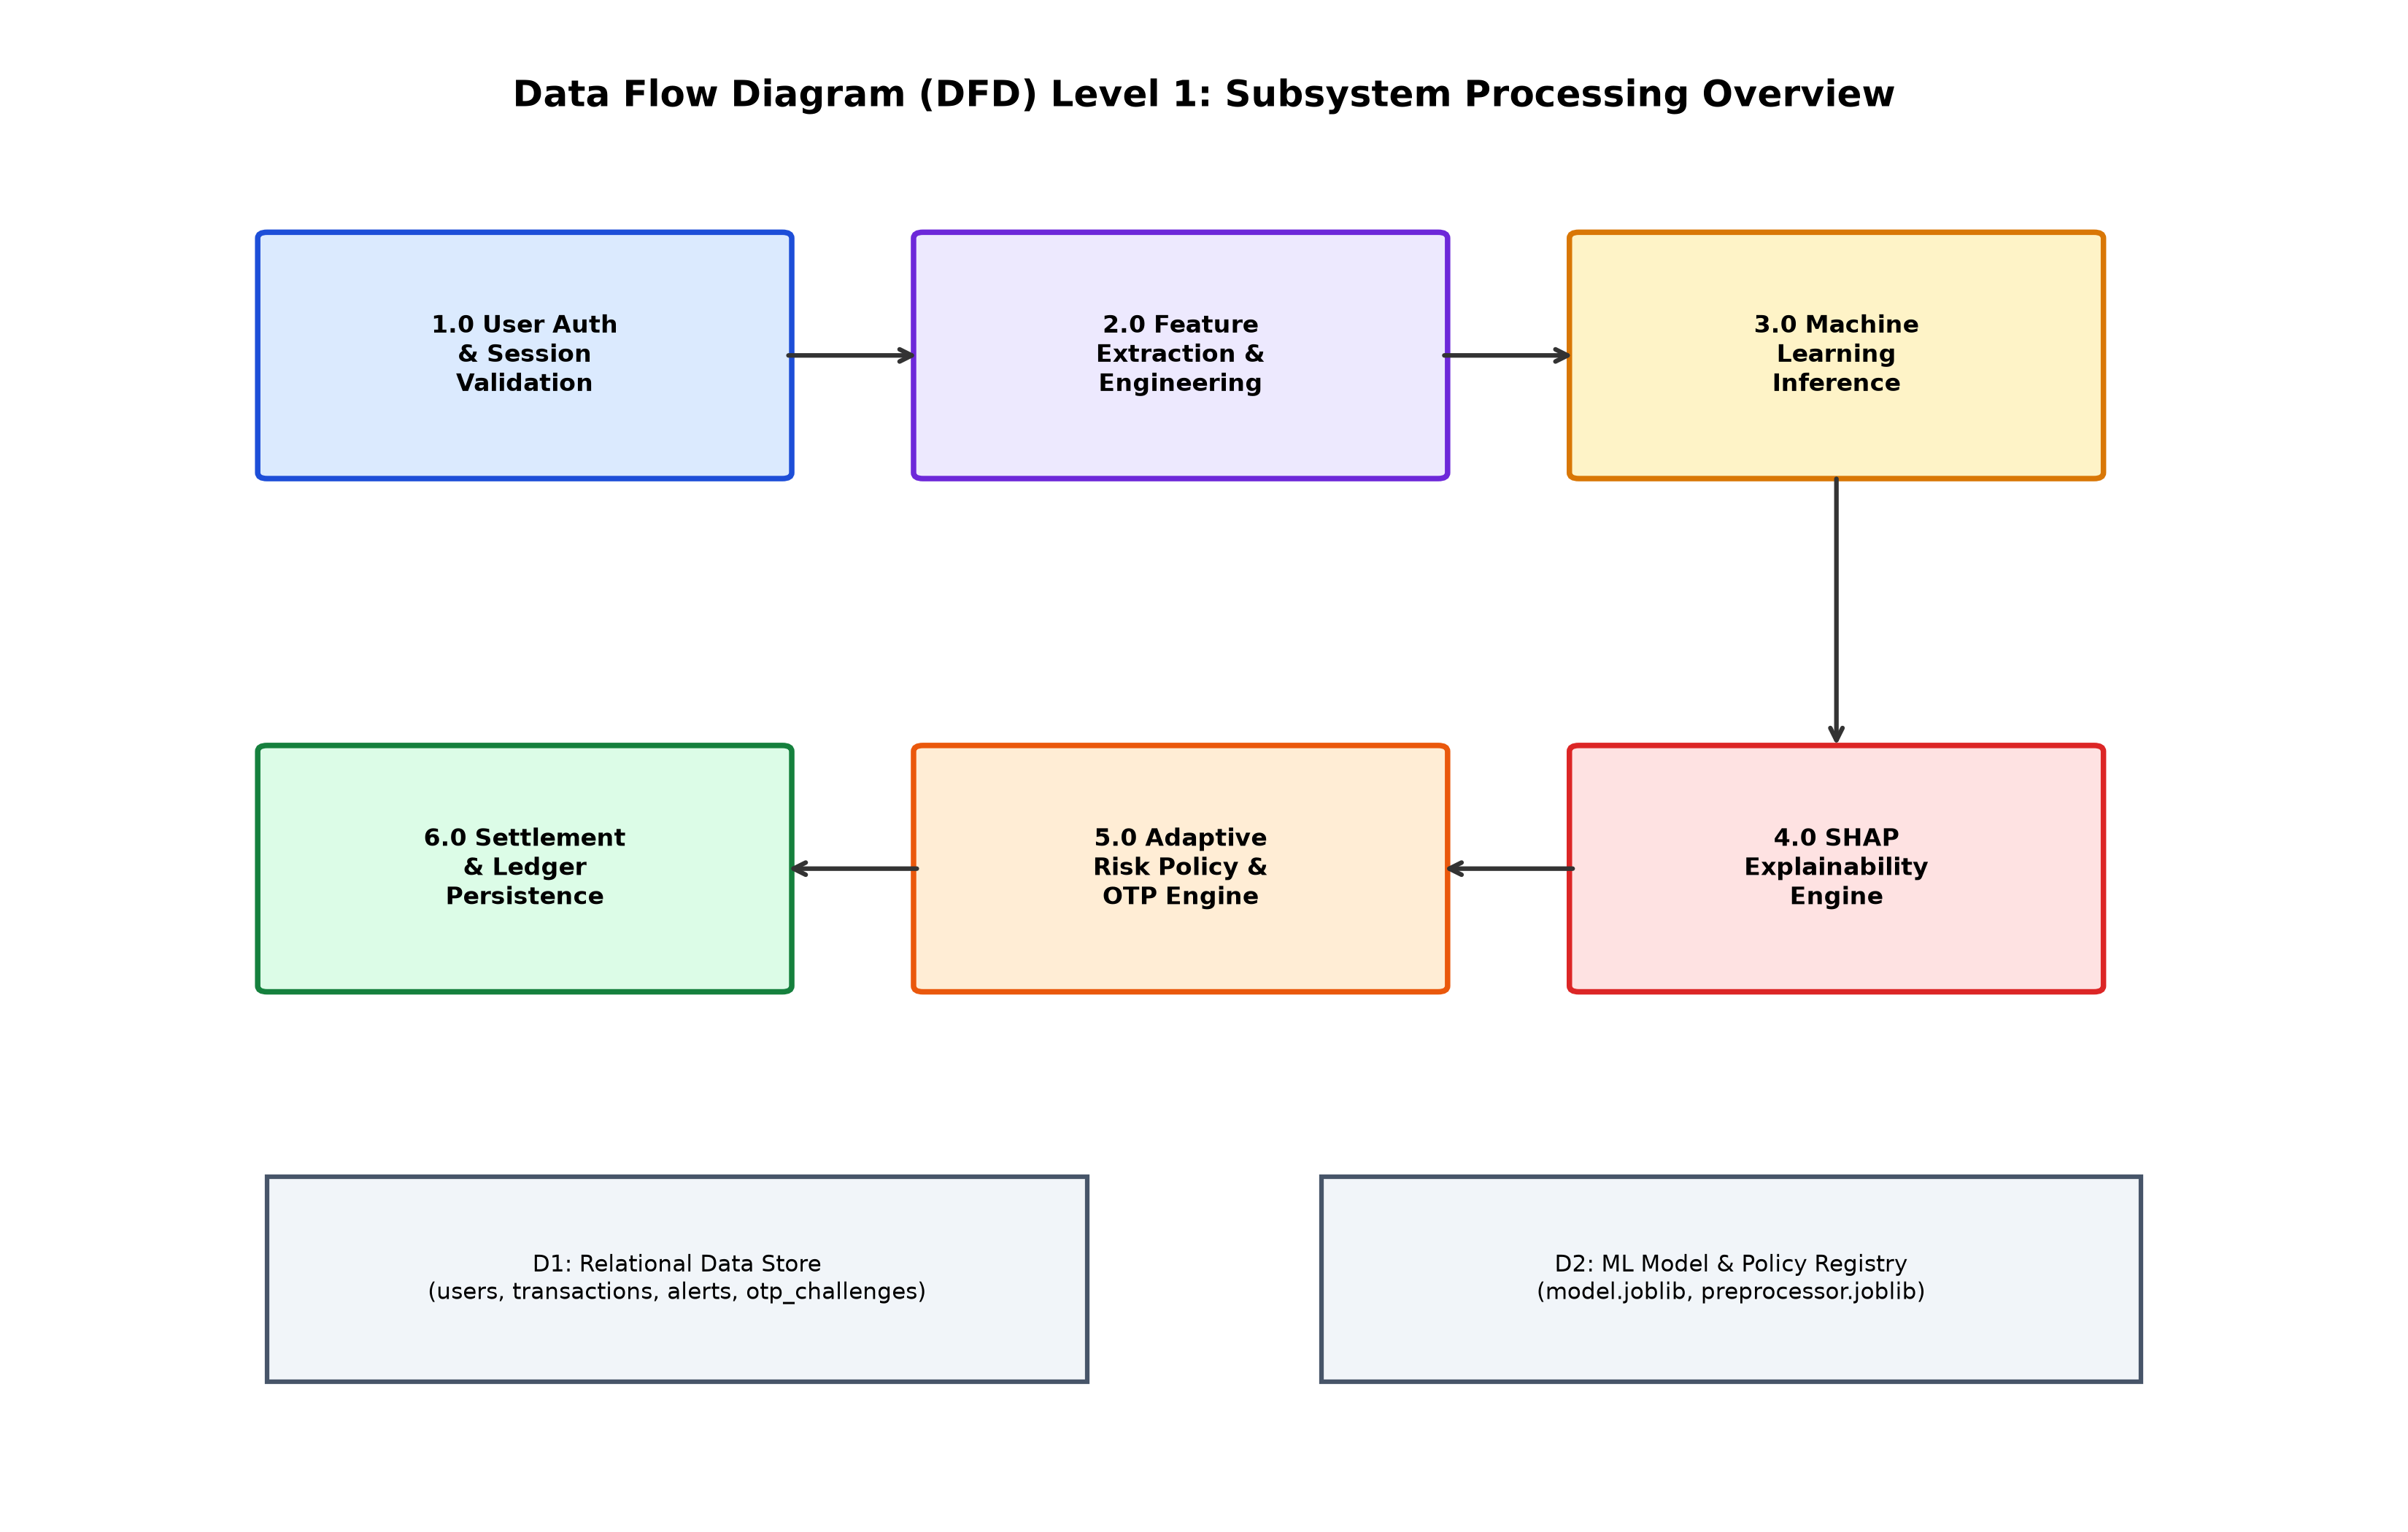
\includegraphics[width=0.88\textwidth]{figures/dfd_level1.png}
    \caption{DFD Level 1: Subsystem Processing Data Flow Diagram}
    \label{fig:dfd_level1}
\end{figure}

\subsection{DFD Level 2 — ML Inference \& Risk Decision Sub-Process}
At Level 2, raw incoming transaction dictionaries are piped through feature sanitization, categorical one-hot encoding, model probability estimation, SHAP attribution decomposition, and policy threshold evaluation, producing the final standardized response payload.
